\documentclass{article}
\usepackage{amsmath}
\usepackage{graphicx}
\begin{document}
\title{Coordinate Geometry Unit Exam: Question 42}
\author{Ana Bhattacharjee}
\date{\today}
\maketitle{}

\begin{center}
The first step is to find the radius of the circle. To do this, we find the distance of the two coordinates to get the diameter and then we divide it by 2 to get the radius.
\begin{align}
  d = \sqrt{(x_2 - x_1)^2 + (y_2 - y_1)^2} \\
  d = \sqrt{(0)^2 + (-4 - 3)^2} = 7 \\
  r = d / 2 \rightarrow 3.5
\end{align}
Now we need to find the center of the circle. The center is just the midpoint of the diameter.
\begin{align}
  M = (\frac{x_1 + x_2}{2}, \frac{y_1 + y_2}{2}) \\
  M = (\frac{0}{2}, \frac{3 - 4}{2}) \\
  M = (0, \frac{-1}{2})
\end{align}
Now with the above information, we can create the equation of the circle.
\begin{align}
  (x)^2 + (y + \frac{1}{2})^2 = 49
\end{align}
\par
The resulting circle is shown in the figure below.
\begin{figure}[!htbp]
  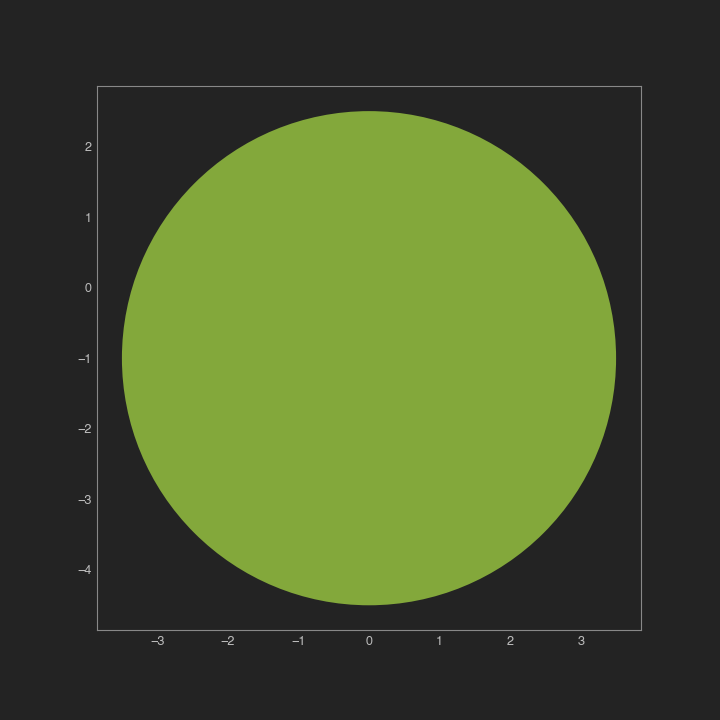
\includegraphics[width=1.0\columnwidth]{circle}
  \caption{Circle Graph}
\end{figure}
\end{center}
\end{document}
